\section{Problem Formulation}\label{sec:prob}
\begin{figure}%[thpb]
	\centering
	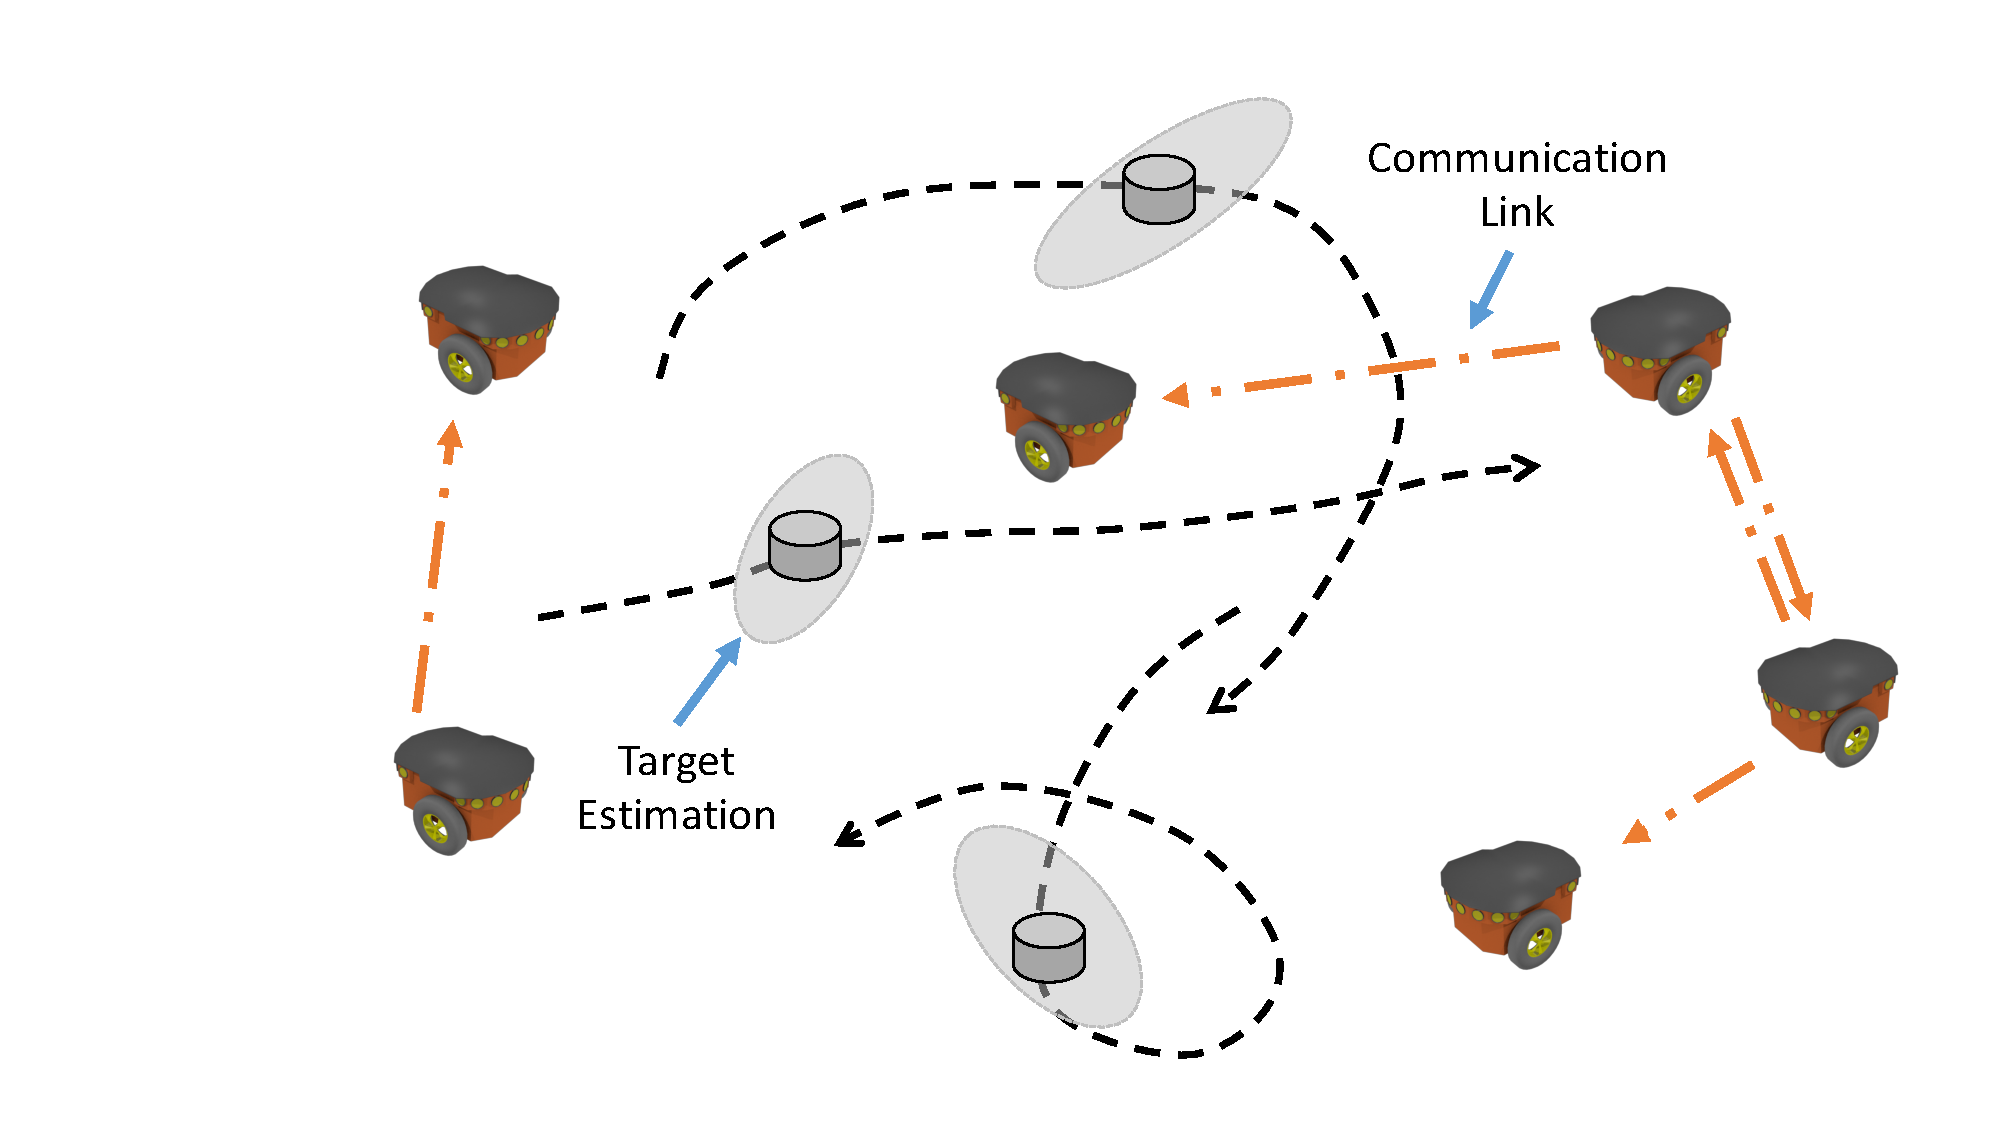
\includegraphics[width=0.45\textwidth]{figures/scenario}
	\caption{Target tracking scenario. The interaction topology is dynamically changing and UGVs can only communicate with neighboring UGVs.}
	\label{fig:scenario}
	%		\vspace{-1em}]
\end{figure}
%	\section{\proto Protocol for Dynamically Changing Interaction Topologies}\label{sec:lifo}
	Consider a network of $N$ UGVs in a bounded two-dimensional space $S$, as shown in \cref{fig:scenario}.
	The interaction topology can be dynamically changing due to limited communication range, team reconfiguration, or intermittently link failure.
	Each UGV is equipped with a sensor for target detection. 
	Due to the limit of communication range, each UGV can only exchange sensor measurements with its local neighbors. 
%	The Bayesian filter is run locally on each UGV based on its own measurements and the received measurements from other UGVs to estimate the target position in $S$.
	Every UGV locally runs a Bayesian filter to estimate the target position in $S$ utilizing its own measurements and the received measurements from other UGVs. 
%	Since this work is focused on the distributed Bayesian filter for target localization, we assume that UGVs' states are accurately known.
%	An illustration of the scenario is shown in \cref{fig:scenario}.
	
	\subsection{Target and Sensor Model}
	%Probabilistic Model of Binary Sensor}
	%In this paper, distributed Bayesian filter is used to estimate the true target position by a network of binary sensors.
	The target motion uses a stochastic discrete-time model: % that can be described by
	
	\begin{equation}
		\small
		\label{eqn:tar_motion_model}
		\xg_{k+1}=f(\xg_k,v_k), %,u^g_k
		%x_{k+1}=A_kx_k+B_ku^g_k+\epsilon,
	\end{equation}\normalsize
	where the superscript $g$ represents the target and $\xg_k\in S$ is the target position at time $k$;
	$v_k$ is the white process noise.
	% and $u^g_k$ is the target control input.
	%$A_k\in\mathbb{R}^{2\times 2},\;B_k\in\mathbb{R}^{2\times 2}$ and $\epsilon$ denotes the process noise.
	
	%Each UGV constantly measures the target position and the 
	The sensor measurement is described by a stochastic model:
	\small\begin{equation}\label{eqn:meas_model}
		z^i_k = h_i(\xg_k,x^i_k)+w^i_k,
	\end{equation}\normalsize
	where the superscript $i\in\left\lbrace 1,\dots,N\right\rbrace$ represents the index of the UGV; $x^i_k\in S$ is the sensor position and $w^i_k$ is the white measurement noise.
	% $x^i_k=[x^i_k;\theta^i_k]$ represents the sensor state, consisting of the sensor position $x^i_k$ and direction $\theta^i_k$.
	The measurement function $h_i$ depends on the type of the sensor. 
	%Let $\mathcal{F}(x^i_k)$ denote the sensor's sensing domain, 
	
%	The conditional probability, denoted by $P(z^i_k|x^g_k;x^i_k)$, of obtaining a certain measurement $z^i_k$ conditioning on the target and sensor states is critical to designing the Bayesian filter \cite{thrun2005probabilistic}. 
	The design of the Bayesian filter relies on the conditional probability of obtaining a certain measurement $z^i_k$ given the target and sensor states, which is denoted by $P(z^i_k|x^g_k;x^i_k)$ \cite{thrun2005probabilistic}. 	
%	We define $P(z^i_k|x^g_k;x^i_k)$ as this conditional probability.
%	 of $z^i_k$ given the sensor state $x^i_k$ and the target state $\xg_k$. 
	The conditional probability $P(z^i_k|x^g_k;x^i_k)$ depends on both $h_i$ and/or $w^i_k$ in \Cref{eqn:meas_model}.
	For example, if $w^i_k$ is a zero-mean Gaussian white noise with covariance $\Gamma_k^i$, $P(z^i_k|x^g_k;x^i_k)$ can be described as $P(z^i_k|x^g_k;x^i_k)=\mathcal{N}(h_i(\xg_k,x^i_k),\Gamma_k^i)$.
%	\small\begin{equation*}%\label{eqn:prob_sensor3}
%		P(z^i_k|x^g_k;x^i_k)=\mathcal{N}(h_i(\xg_k,x^i_k),\Gamma_k^i).
%	\end{equation*}\normalsize
	For non-Gaussian noise, such as Poisson noise or Cauchy noise \cite{kitagawa1996monte}, $P(z^i_k|x^g_k;x^i_k)$ can also be similarly defined (for the purpose of simplicity, $P(z^i_k|x^g_k;x^i_k)$ is shorted as $P(z^i_k|x^g_k)$ for the rest of the paper). 
	It should be noted that this work is not confined to any specific distribution of the noise.
	The measurement function $h_i$ for several typical sensors are listed as follows \cite{bishop2010optimality}:
	
	\textbf{Range-only sensors:} 
	%when the target is within the sensor's sensing domain, 
	$h_i$ is a function of the relative Euclidean distance between the sensor and the target:
	%\begin{subequations}
	%	\begin{align}
	\small\begin{equation*}%\label{eqn:ran_only}
		h_i(\xg_k,x^i_k)=\|\xg_k-x^i_k\|_2,
	\end{equation*}	\normalsize
	%\begin{equation}\label{eqn:ran_only}
	%h_i(\xg_k,w^i_k;x^i_k)=
	%\begin{cases}
	%\|\xg_k-x^i_k\|_2+w^i_k\; &\text{if}\, \xg_k\in\mathcal{F}(x^i_k)\\
	%\emptyset\; &\text{if}\, \xg_k\notin\mathcal{F}(x^i_k)
	%\end{cases},
	%\end{equation}		
	where $\|\cdot\|_2$ is the Euclidean distance in $S$.
	%		w^i_k&\sim\mathcal{N}(0,\sigma^i),
	%	\end{align}
	%\end{subequations}
	
	\textbf{Bearing-only sensors:} 
	%when the target is within the sensor's sensing domain, 
	$h_i$ is a function of the relative bearing between the sensor and the target:
	\small\begin{equation*}
		h_i(\xg_k,x^i_k)=\measuredangle (\xg_k-x^i_k),
	\end{equation*}\normalsize
	%\begin{equation}
	%h_i(\xg_k,w^i_k;x^i_k)=
	%\begin{cases}
	%\measuredangle (\xg_k-x^i_k)+w^i_k\; &\text{if}\, \xg_k\in\mathcal{F}(x^i_k)\\
	%\emptyset\; &\text{if}\, \xg_k\notin\mathcal{F}(x^i_k)
	%\end{cases},
	%\end{equation}
	where $\measuredangle$ denotes the angle from the sensor to the target.
	
	\textbf{Range-bearing sensors:} $h_i$ includes both the relative distance and bearing: % between the sensor and the target:
	\small\begin{equation*}
		h_i(x^g_k,x^i_k)=x^g_k-x^i_k.
	\end{equation*}\normalsize
	
%	\subsection{Target and Sensor Model}
%	The target motion takes a deterministic discrete-time model:	
%	\begin{equation}
%		\small
%		\label{eqn:tar_motion_model}
%		x^g_{k+1}=f(x^g_k),
%	\end{equation}\normalsize
%	where $x^g_k\in \mathbb{R}^{2}$ denotes the target position at time $k$; $u^g_k$ represents the control input of the target.
%	
%	Each UGV constantly measures the target position and the sensor measurement of $i\thi$ UGV can be described by a stochastic model:
%	\begin{equation}
%		z^i_k = g_i(x^g_k,w^i_k;y^i_k),
%	\end{equation}
%	where $w^i_k$ is the white measurement noise and $y^i_k=[x^i_k;\theta^i_k]$ represents the sensor state, consisting of the sensor position $x^i_k$ and direction $\theta^i_k$.
%	$g_i$ depends on the type of the sensor. Let $\mathcal{F}(y^i_k)$ denote the sensor field of view (FOV), $g_i$ for several typical sensor types can be defined as follows:
%	
%	\textbf{Range-only sensors:} when the target is within the sensor's FOV, the measurement only depends on the relative distance between the sensor and the target.
%	\begin{equation*}%\label{eqn:ran_only}
%		h_i(\xg_k,x^i_k)=\|\xg_k-x^i_k\|_2,
%	\end{equation*}	
%%	\begin{equation}
%%		g_i(x^g_k,w^i_k;x^i_k)=
%%		\begin{cases}
%%			\|x^g_k-x^i_k\|_2+w^i_k\; &\text{if}\, x^g_k\in\mathcal{F}(y^i_k),\\
%%			\emptyset\; &\text{if}\, x^g_k\notin\mathcal{F}(y^i_k).
%%		\end{cases}
%%	\end{equation}
%	
%	\textbf{Bearing-only sensors:} when the target is within the sensor's FOV, the measurement only depends on the relative bearing between the sensor and the target.
%	\begin{equation}
%		g_i(x^g_k,w^i_k;x^i_k)=
%		\begin{cases}
%			\measuredangle (x^g_k-x^i_k)+w^i_k\; &\text{if}\, x^g_k\in\mathcal{F}(y^i_k),\\
%			\emptyset\; &\text{if}\, x^g_k\notin\mathcal{F}(y^i_k).
%		\end{cases}
%	\end{equation}
%	
%	\textbf{Range-bearing sensors:} $h_i$ includes both the relative distance and bearing: % between the sensor and the target:
%	\begin{equation*}
%		h_i(x^g_k,x^i_k)=x^g_k-x^i_k.
%	\end{equation*}
%	
%%	\textbf{Range-bearing sensors:} when the target is within the sensor's FOV, the measurement is the relative distance and bearing between the sensor and the target.
%%	\begin{equation}
%%		g_i(x^g_k,w^i_k;x^i_k)=
%%		\begin{cases}
%%			x^g_k-x^i_k+w^i_k\; &\text{if}\, x^g_k\in\mathcal{F}(y^i_k),\\
%%			\emptyset\; &\text{if}\, x^g_k\notin\mathcal{F}(y^i_k).
%%		\end{cases}
%%	\end{equation}
%		
%	A probabilistic sensor model that describes the conditional probability of a certain measurement given sensor and target state is a key component for Bayesian filtering.
%	We define a likelihood function to represent the probability of the target being detected by a sensor:
%	\small\begin{equation}\label{eqn:prob_sensor1}
%		p^i_{1,k}=P(z^i_k\neq\emptyset|x^g_k;x^i_k)\in \left[0,1\right],\; x^g_k\in S,
%	\end{equation}\normalsize
%	where $x^i_k$ is the $i\thi$ sensor's position.
%	%; $X^g$ represents the set of all possible target positions.
%	Correspondingly, the likelihood function for no target being detected is:
%	\small\begin{equation}\label{eqn:prob_sensor0}
%		p^i_{0,k}=P(z^i_k=\emptyset|x^g_k;x^{i}_k)=1-p^i_{1,k}.
%	\end{equation}\normalsize
%	%\Cref{eqn:bin_sensor} actually defines a binary sensor model parameterized by $x^g_k$ and $x^R_k$.
%	
%	The combination of \Cref{eqn:prob_sensor1} and \Cref{eqn:prob_sensor0} forms the probabilistic model for a sensor.
%	If $w^i_k$ is a zero-mean Gaussian white noise, then the probabilistic sensor model can be described as
%	\begin{equation}		
%		\begin{cases}
%			p^i_{1,k}\sim\mathcal{N}(\bar{z}^i_k,\Sigma^i_k) & \text{if}\,x^g_k\in\mathcal{F}(y^i_k)\\
%			p^i_{1,k}=0 & \text{if}\,x^g_k\in\mathcal{F}(y^i_k),
%		\end{cases}
%	\end{equation}
%	where $\bar{z}^i_k$ is the nominal value of the measurement and equals $\|x^g_k-x^i_k\|$ and $\measuredangle(x^g_k-x^i_k)$ for range-only and bearing-only sensors, correspondingly.
%	
%	Consequently,
%	\begin{equation}
%		p^i_{0,k}=
%		\begin{cases}
%			0 & \text{if}\,x^g_k\in\mathcal{F}(y^i_k)\\
%			1 & \text{if}\,x^g_k\in\mathcal{F}(y^i_k).
%		\end{cases}
%	\end{equation}
	
%	For the purpose of simplicity, we will not explicitly write $x^{i}_k$ in the sensor model (\Cref{eqn:prob_sensor1,eqn:prob_sensor0}) for the rest of the paper.
	
	\begin{rem}
		Given the knowledge of current target and UGV positions, the current measurement by each UGV can be considered conditionally independent from its own past measurements and those by other UGVs \cite{bourgault2003optimal}.
	\end{rem}
	
%	\begin{rem} 
%		The proposed {\proto} protocol and the consistency property to be described in \cref{sec:\proto-dbf} are applicable for general sensors, not limited to the ones described in this section. In addition, they do not rely on the Gaussian noise assumption.
%	\end{rem}
	
	\subsection{Graphical Model of Interaction Topology}
	%The UGV network is always assumed to be connected, i.e., there exists a path, either direct or indirect, between every pair of UGVs.
	%Under this assumption, consider an undirected and fixed graph 
	We consider a simple\footnote{A (directed/undirected) graph $G=(V,E)$ is \textit{simple} if it has no self-loops (i.e., $\left( i,j\right)\in E\,\text{only if } i\neq j$) or multiple edges with the same source and target nodes (i.e., $E$ only contains distinct elements).} graph $G=(V,E)$ to represent the interaction topology of N networked UGVs, where the vertex set $V=\left\lbrace 1,\dots,N\right\rbrace $ represents the index set of UGVs and $E=V\times V$ denotes the edge set. 
	For the purpose of narrative simplicity, we use directed graphs to describe our approach in this work.
%	The approach can conveniently apply to undirected graphs, which can be treated as bidirectional directed graphs.
	The undirected graphs can be treated as bidirectional directed graphs.
	
	The \textit{adjacency matrix} $A=\left[ a_{ij}\right] $ of the graph $G$ describes the interaction topology:
	\small\begin{equation*}
		a_{ij}=\begin{cases}
			1& \text{if}\;\left(i,j\right)\in E\\
			0& \text{if}\;\left(i,j\right)\notin E
		\end{cases},
	\end{equation*} \normalsize
	where $a_{ij}$ is the entry on the $i\thi$ row and $j\thi$ column of the adjacency matrix. 
	The notation $a_{ij}=1$ indicates that the $i\thi$ UGV can directly communicate to the $j\thi$ UGV and $a_{ij}=0$ indicates no direct communication from $i$ to $j$.
%	 a communication link exists from the $i\thi$ to $j\thi$ UGV and $m_{ij}=0$ indicates no communication from $i$ to $j$.
	 A directed graph is \textit{strongly connected} if there is a directed path connecting any two arbitrary vertices in $V$. %\footnote{An undirected graph with this property is called a \textit{connected} graph.}.
%	\cref{fig:com_topo} illustrates three types of typical simple directed topologies: ring \cite{lawton2003decentralized}, line \cite{liu2010simple}, and star \cite{thatte2008sensor}. 
%	All of them are represented by simple and undirected graphs.
	
%	The interaction topology can be dynamically changing due to limited communication range, varying team formation or link failure.
%	Let $\bar{G}=\left\lbrace G_1,G_2,\dots,G_L\right\rbrace $ denote the set of all possible simple and undirected graphs defined for the network of UGVs.
%	Let $\bar{G}$ denote the set of all possible simple and undirected graphs defined for the network of UGVs.
%	Let $\bar{G}$ denote the set of all possible simple directed graphs\footnote{For undirected graphs, we consider the set of simple undirected graphs.} defined over the network of UGVs.
%	It is easy to know that $\bar{G}$ has finite elements.
%	The adjacency matrix associated with a graph $G_l\in\bar{G}$ is denoted as $A_l=[a^l_{ij}]$.	
	Define the \textit{union} of a collection of simple directed graphs 
	%\footnote{For undirected graphs, we consider the set of simple undirected graphs.} 
%	\small$\lb G_{i_1},G_{i_2},\dots,G_{i_l} \rb$\normalsize
	as the graph with the vertices in $V$ and the edge set given by the union of each member's edge sets.
%	 of \small$G_{i_j},\,j=1\dots,l$\normalsize.
	Such collection is \textit{jointly strongly connected} if the union of its members forms a strongly connected graph.
%	\footnote{For undirected graphs, such collection is \textit{jointly connected} \cite{jadbabaie2003coordination}.}.
%	We define the concept of neighbors in a UGV network.
%	\todohere{note that the definition for neighbor here means neighbors who can receive robot $i$'s CB, so it's outbound neighbors for directed graph.}
	We use $G_{k}$ to represent the interaction topology of time $k$ and define the \textit{\inbhd} and \textit{\onbhd} of the $i\thi$ UGV under $G_{k}$ as the set \small$\N^\text{in}_i(G_{k})=\left\lbrace j|a^k_{ji}=1,\,j\in V\right\rbrace $\normalsize and  \small$\N^\text{out}_i(G_{k})=\left\lbrace j|a^k_{ij}=1,\,j\in V\right\rbrace $\normalsize. %\left\lbrace1,\dots,N \right\rbrace 
	All UGVs in $\N_i(G_{k})$ can directly receive information from the $i\thi$ UGV via the single hopping.
%	The \textit{\anbhd} is defined as $\mathcal{Q}_i(G_{l})$ that contains indices of UGVs whose information can be received by the $i\thi$ UGV, possibly via multi-hopping, given a specific data exchange protocol and the interaction topology $G_{l}$. 
%	Note that in general $\mathcal{N}_i(G_{l})\subseteq\mathcal{Q}_i(G_{l})$.
	%but when only single-hopping is allowed, $\mathcal{N}_i=\mathcal{Q}_i$. 